\documentclass[11pt,a4paper]{article}

\usepackage[T1]{fontenc}
\usepackage[utf8]{inputenc}
\usepackage[french]{babel} % Global stuff set to french
\usepackage[margin=2.5cm]{geometry} % The margin of the page
% \usepackage{amsmath}  % to include math formulas
\usepackage{graphicx} % to include pictures
\usepackage[hidelinks]{hyperref} % To include hyperlinks in a PDF
\usepackage{fancyhdr} % to be able to make the page fancy looking
\usepackage{appendix} % To make appendixes
\usepackage{color} % For text colors
\usepackage{palatino} % Change font
% \usepackage{tabularx}
\usepackage{subcaption}
\usepackage{enumitem}
\usepackage{changepage}
\usepackage[nonumberlist, nopostdot, numberedsection, toc]{glossaries}
\usepackage{imakeidx}
\usepackage{rotating}
\makeindex
\makenoidxglossaries

%% Fancy layout
\pagestyle{fancy}
\lhead{Projet d'année - Wizard Poker}
\chead{}
\rhead{Groupe 2}
\lfoot{}
\cfoot{}
\rfoot{Page \thepage}
\renewcommand{\headrulewidth}{0.4pt}
\renewcommand{\footrulewidth}{0.4pt}



%%% Glossary

\newglossaryentry{deck}{
  name=Deck,
  description=est un ensemble de 20 cartes constitué par un joueur à partir de sa collection afin d'être utilisé par ce dernier lors d'un duel.
}

\newglossaryentry{carte}{
  name=Carte,
  description=peut appartenir à la collection d'un joueur et est utilisée lors d'une partie. Une carte peut être de deux types : créature ou sort.,
}

\newglossaryentry{app}{
  name=Application/système,
  description=constitue le jeu Wizard Poker à développer.
}

\newglossaryentry{collection}{
  name=Collection,
  description=est un ensemble qui contient toutes les cartes disponibles et
  connues par un joueur.
}

\newglossaryentry{tchat}{
  name=Tchat,
  description=est la messagerie instantanée permettant à deux personnes de
  s'échanger des messages écrits.
}

\newglossaryentry{visiteur} {
  name=Visiteur,
  description=est une personne n'ayant pas (encore) de compte.
}

\newglossaryentry{sort} {
  name=Sort,
  description=est un type de carte ayant un coût en énergie et un effet spécial.
}

\newglossaryentry{monstre} {
  name=Monstre,
  description={est un type de carte ayant un coût en énergie, une valeur d'attaque et des
  points de vie, ainsi que, optionnellement,  un effet spécial.}
}

\newglossaryentry{energie} {
  name=Énergie,
  description={est une quantité (de type nombre entier) représentant le coût pour jouer une carte.}
}

\newglossaryentry{defausse} {
  name=Défausser,
  description={Action de se débarrasser d'une carte qui sera elle-même placée dans une défausse en vue d'être récupérée par le joueur qui la possède.}
}

\newglossaryentry{pseudo} {
  name=Pseudo,
  description={Nom qu'une personne peut prendre en jeu afin de remplacer son vrai prénom.}
}


%%% --- %%% --- DOCUMENT START --- %%% --- %%%
\begin{document}
\begin{titlepage}

\topskip0pt
\begin{center}
    \vspace*{\fill}
        \hrule
        \vspace*{2pt}
        \hrule
        \vspace*{15pt}
        \textsc{\Huge{INFO-F106 : Projet d'année \\\vspace*{8pt} Rappport intermédiaire}}
        \vspace*{15pt}
        \hrule
        \vspace*{2pt}
        \hrule
  \vspace*{\fill}
\end{center}
\null
\vfill
  
\large{Mardi 16 décembre 2014} \hfill \large{Carlos Requena López - \emph{410031}}

\end{titlepage}
\pagestyle{empty}
\tableofcontents
\newpage
%%% Counting pages now %%%
\pagestyle{fancy}

\setcounter{page}{1}

\section{Introduction}
\label{sec:intro}

\subsection{But du projet}
\label{sec:but}

Dans le cadre du projet d'analyse et méthodes et de systèmes
d'exploitation, il est demandé d'implémenter un jeu de cartes en ligne.

\medbreak

\index{Créature}
\index{Sort}
Ce projet devra fournir un jeu de cartes symétrique où deux joueurs
pourront s'affronter et gagner des points pour un classement
général. Chaque joueur disposera d'un ensemble de cartes avec lesquelles
il pourra affronter ses adversaires. Ces cartes pourront être des
créatures pouvant attaquer et des cartes de type
sort qui lanceront des événements spéciaux.

\medbreak

Le système fournira à l'utilisateur une interface intuitive, un gestionnaire
d'amis, un service de tchat pour pouvoir rester en contact avec eux ainsi
qu'un classement général où chaque joueur pourra comparer ses résultats avec
ceux des autres.

\medbreak

Le Wizard Poker sera disponible pour n'importe quel joueur enregistré
afin de jouer contre d'autres joueurs (également enregistrés), lui
permettant d'essayer de gagner des places dans le classement
général. Il permettra aussi à des visiteurs de s'enregistrer en tant que nouveaux joueurs.


\medbreak

\index{Deck}
Dans le cas d'une inscription, le nouveau joueur recevra ses premières
cartes. De plus, tout joueur sera invité à confectionner son premier
Deck avant d'affronter son premier adversaire.

\subsection{Historique du document}
\label{sec:hist}

Voir table \ref{tab:hist}


\begin{table}[h]
  \centering
  \begin{tabular}[ht]{|l|l|l|p{18em}|}
    \hline
    \textbf{Version}
    & \textbf{Auteur}
    & \textbf{Date modification}
    & \textbf{Description des changements}\\ \hline \hline
    v2.0 & Team & 26/2/16 & Delivrable phase 2 \\ \hline
    v1.5 & ??? & ?/?/? & ??? \\ \hline
    v1.4 & Maxime Dewit & 25/2/16 & UML \\ \hline
    v1.3 & Carlos Requena & 25/2/16 & Exigences fonctionnelles système
    \\ \hline
    v1.2 & Corentin Candeur & 24/2/16 & UML \\ \hline
    v1.1 & Rémy Detobel & 24/2/16 & UML \\ \hline
    v1.0 & Team & 18/12/15 & Delivrable phase 1 \\ \hline
    v0.8 & Rémy Detobel & 18/12/15 & Correction de la partie ``Besoins de l'utilisateur'' \\ \hline
    v0.7 & Lucie Borremans & 17/12/15 & Relecture, mise en page, corrections \\ \hline
     v0.6 & Corentin Candeur & 16/12/15 & Deuxième relecture, corrections orthographiques/syntaxiques et diverses petites corrections \\ \hline
    v0.5 & Rémy Detobel & 14/12/15 & Première relecture, diverses petites corrections \\ \hline
    v0.4 & Carlos Requena  & 13/12/15 & Ajout d'un système de glossaire \\ \hline
    v0.3 & Rémy et Lucie  & 11/12/15 & Ajout de diagrammes, ajout de ``Exigences du domaine'' \\ \hline
    v0.2 & Amin et Maxime & 10/12/15 & Ajout de la partie ``Exigences fonctionnelles''\\ \hline
    v0.1 & Jonas et Raphaël & 10/12/15 & Ajout de la partie ``But du projet''\\ \hline
    v0.0 & Carlos Requena & 26/11/15 & Mise en place du document. Ajout des diagrammes réalisés en groupe le 25/11/15.\\ \hline
  \end{tabular}
  \caption{Changements apportés au document.}
  \label{tab:hist}
\end{table}


\glsaddall
\printnoidxglossaries


\section{Besoins de l'utilisateur}
\label{sec:besoins}

En tant que jeu de cartes fantastique en ligne, le Wizard Poker doit fournir un minimum de services. Avant de pouvoir jouer, le joueur devra donc se créer un compte et se connecter à celui-ci.

\medbreak

\index{Collection}
Lors de la création d'un compte, le joueur recevra 100 cartes dans sa \gls{collection}.  À chaque fois qu'il gagnera une partie, il gagnera également une carte.  Cette carte sera choisie aléatoirement parmi toutes les cartes disponibles dans le jeu.  Notons qu'une même carte peut se retrouver plusieurs fois dans la \gls{collection} d'un joueur.

\medbreak
\index{Cartes}
\index{Sort}
\index{Défausser}
\index{Monstre}
Il existe deux types de \gls{carte}s dans le jeu. D'une part, on retrouve les cartes \gls{sort}s qui sont des cartes à effets. Cependant, dès qu'une carte \gls{sort} aura été jouée, elle sera directement \gls{defausse}e (=retirée du jeu) et son effet sera immédiat (dans la majorité des cas). D'autre part, on retrouve les cartes \gls{monstre}s qui sont des cartes devant être posées sur le plateau par le joueur. Pour pouvoir attaquer avec les monstres, ces derniers doivent être sur le terrain au minimum depuis un tour. Certains monstres peuvent aussi avoir plusieurs effets spéciaux.

\medbreak

\index{Deck}
Avec cette \gls{collection} le joueur pourra créer un, voire, des \gls{deck}s.  Un \gls{deck} est composé d'exactement 20 cartes.  De plus, il peut y avoir au maximum deux fois la même carte dans un \gls{deck} mais seulement si le joueur possède au moins deux exemplaires de la-dite carte dans sa \gls{collection}.  Les Decks sont indépendants.  Cela signifie qu'une carte peut appartenir à plusieurs decks.

\medbreak

\index{Énergie}
Toutes les cartes ayant un coût en \gls{energie}, celle-ci est primordiale dans un duel. En effet, c'est grâce à sa jauge d'énergie que le joueur pourra jouer ses cartes. Pour cela, il faut que le coût en énergie de la carte soit inférieur ou égal aux points d'énergie encore disponibles pendant son tour de jeu.

\medbreak

\index{Tchat}
Le Wizard Poker étant un jeu en ligne, il permet donc de mettre les joueurs en contact. Premièrement, chaque joueur a la possibilité de gérer une liste d'amis. Un joueur pourra donc ajouter et retirer des amis à sa liste. Mais il pourra également jouer des duels avec ses amis. Deuxièmement, le Wizard Poker propose un système de \gls{tchat} permettant à deux joueurs étant amis de s'échanger des messages.  Ce tchat est disponible à tout moment.

\medbreak

Lorsqu'un joueur souhaitera lancer une partie, le programme choisira arbitrairement une personne connectée pour lancer un duel. Il est à noter que si le joueur ne possède pas encore de deck, il sera invité à créer son deck et pourra ensuite jouer. Sinon, il devra simplement choisir un deck avant de commencer la partie.

\medbreak

Lors de chaque début de partie, chaque joueur commence avec 20 points de vie, 1 point d'énergie et 5 cartes en main. À chaque début de tour, le joueur en question gagnera un point d'énergie supplémentaire jusqu'à atteindre un maximum de 10 points.

\medbreak

En ce qui concerne le mode de jeu, il s'agit ici d'un jeu de cartes au tour par tour.  Cela signifie que chaque utilisateur joue à son tour.  Les joueurs ne jouent donc jamais en même temps.  Lorsque vient le tour d'un joueur, celui-ci se voit offrir le choix entre plusieurs actions. Il peut:

\index{Sort}
\begin{itemize}
 \item[\textbullet] jouer une carte Sort;
 \item[\textbullet] poser une carte Monstre;
 \item[\textbullet] demander à une carte monstre d'attaquer soit une carte Monstre adverse, soit le joueur adverse lui-même ;
 \item[\textbullet] finir son tour.
\end{itemize}

Pour pouvoir demander à une carte monstre d'attaquer il faut que celle-ci ait été placée au minimum au tour précédent.  Lorsqu'une carte monstre attaque un élément adverse (que ça soit une carte monstre ou le joueur adverse) l'élément attaqué perd un nombre de points de vie égal à la valeur d'attaque de la carte attaquante. Lorsqu'une carte monstre a 0 (ou moins) point de vie, elle meurt et est défaussée.

\medbreak


Les joueurs pourront chacun poser au maximum 7 cartes monstres sur le plateau ainsi qu'avoir au maximum 7 cartes en main. Si à la fin du tour du joueur, ce dernier a plus de 7 cartes en main, il devra décider de quelle(s) carte(s) il souhaite se défausser. De plus, si un joueur a épuisé toutes les cartes de son deck, il perdra 5 points de vie à chaque début de tour.

\medbreak

Une partie se termine lorsqu'un des deux joueurs arrive à 0 (ou moins) point de vie.  Celui-ci aura donc perdu la partie.  Par contre, le joueur vainqueur recevra une carte qui sera choisie aléatoirement parmi toutes les cartes disponibles dans le jeu.


\subsection{Exigences fonctionnelles}

Les exigences fonctionnelles ne sont autres, ici, que celles présentées dans la Figure \ref{fig:usecasebesoin}. Nous y voyons, d'ailleurs deux types d'acteurs agissant sur le système : le Joueur et le \gls{visiteur}. Les actions possibles par ceux-ci sur l'application sont décrites ci-dessous.

\label{sec:exi-fonc}
\begin{figure}[ht]
  \centering
  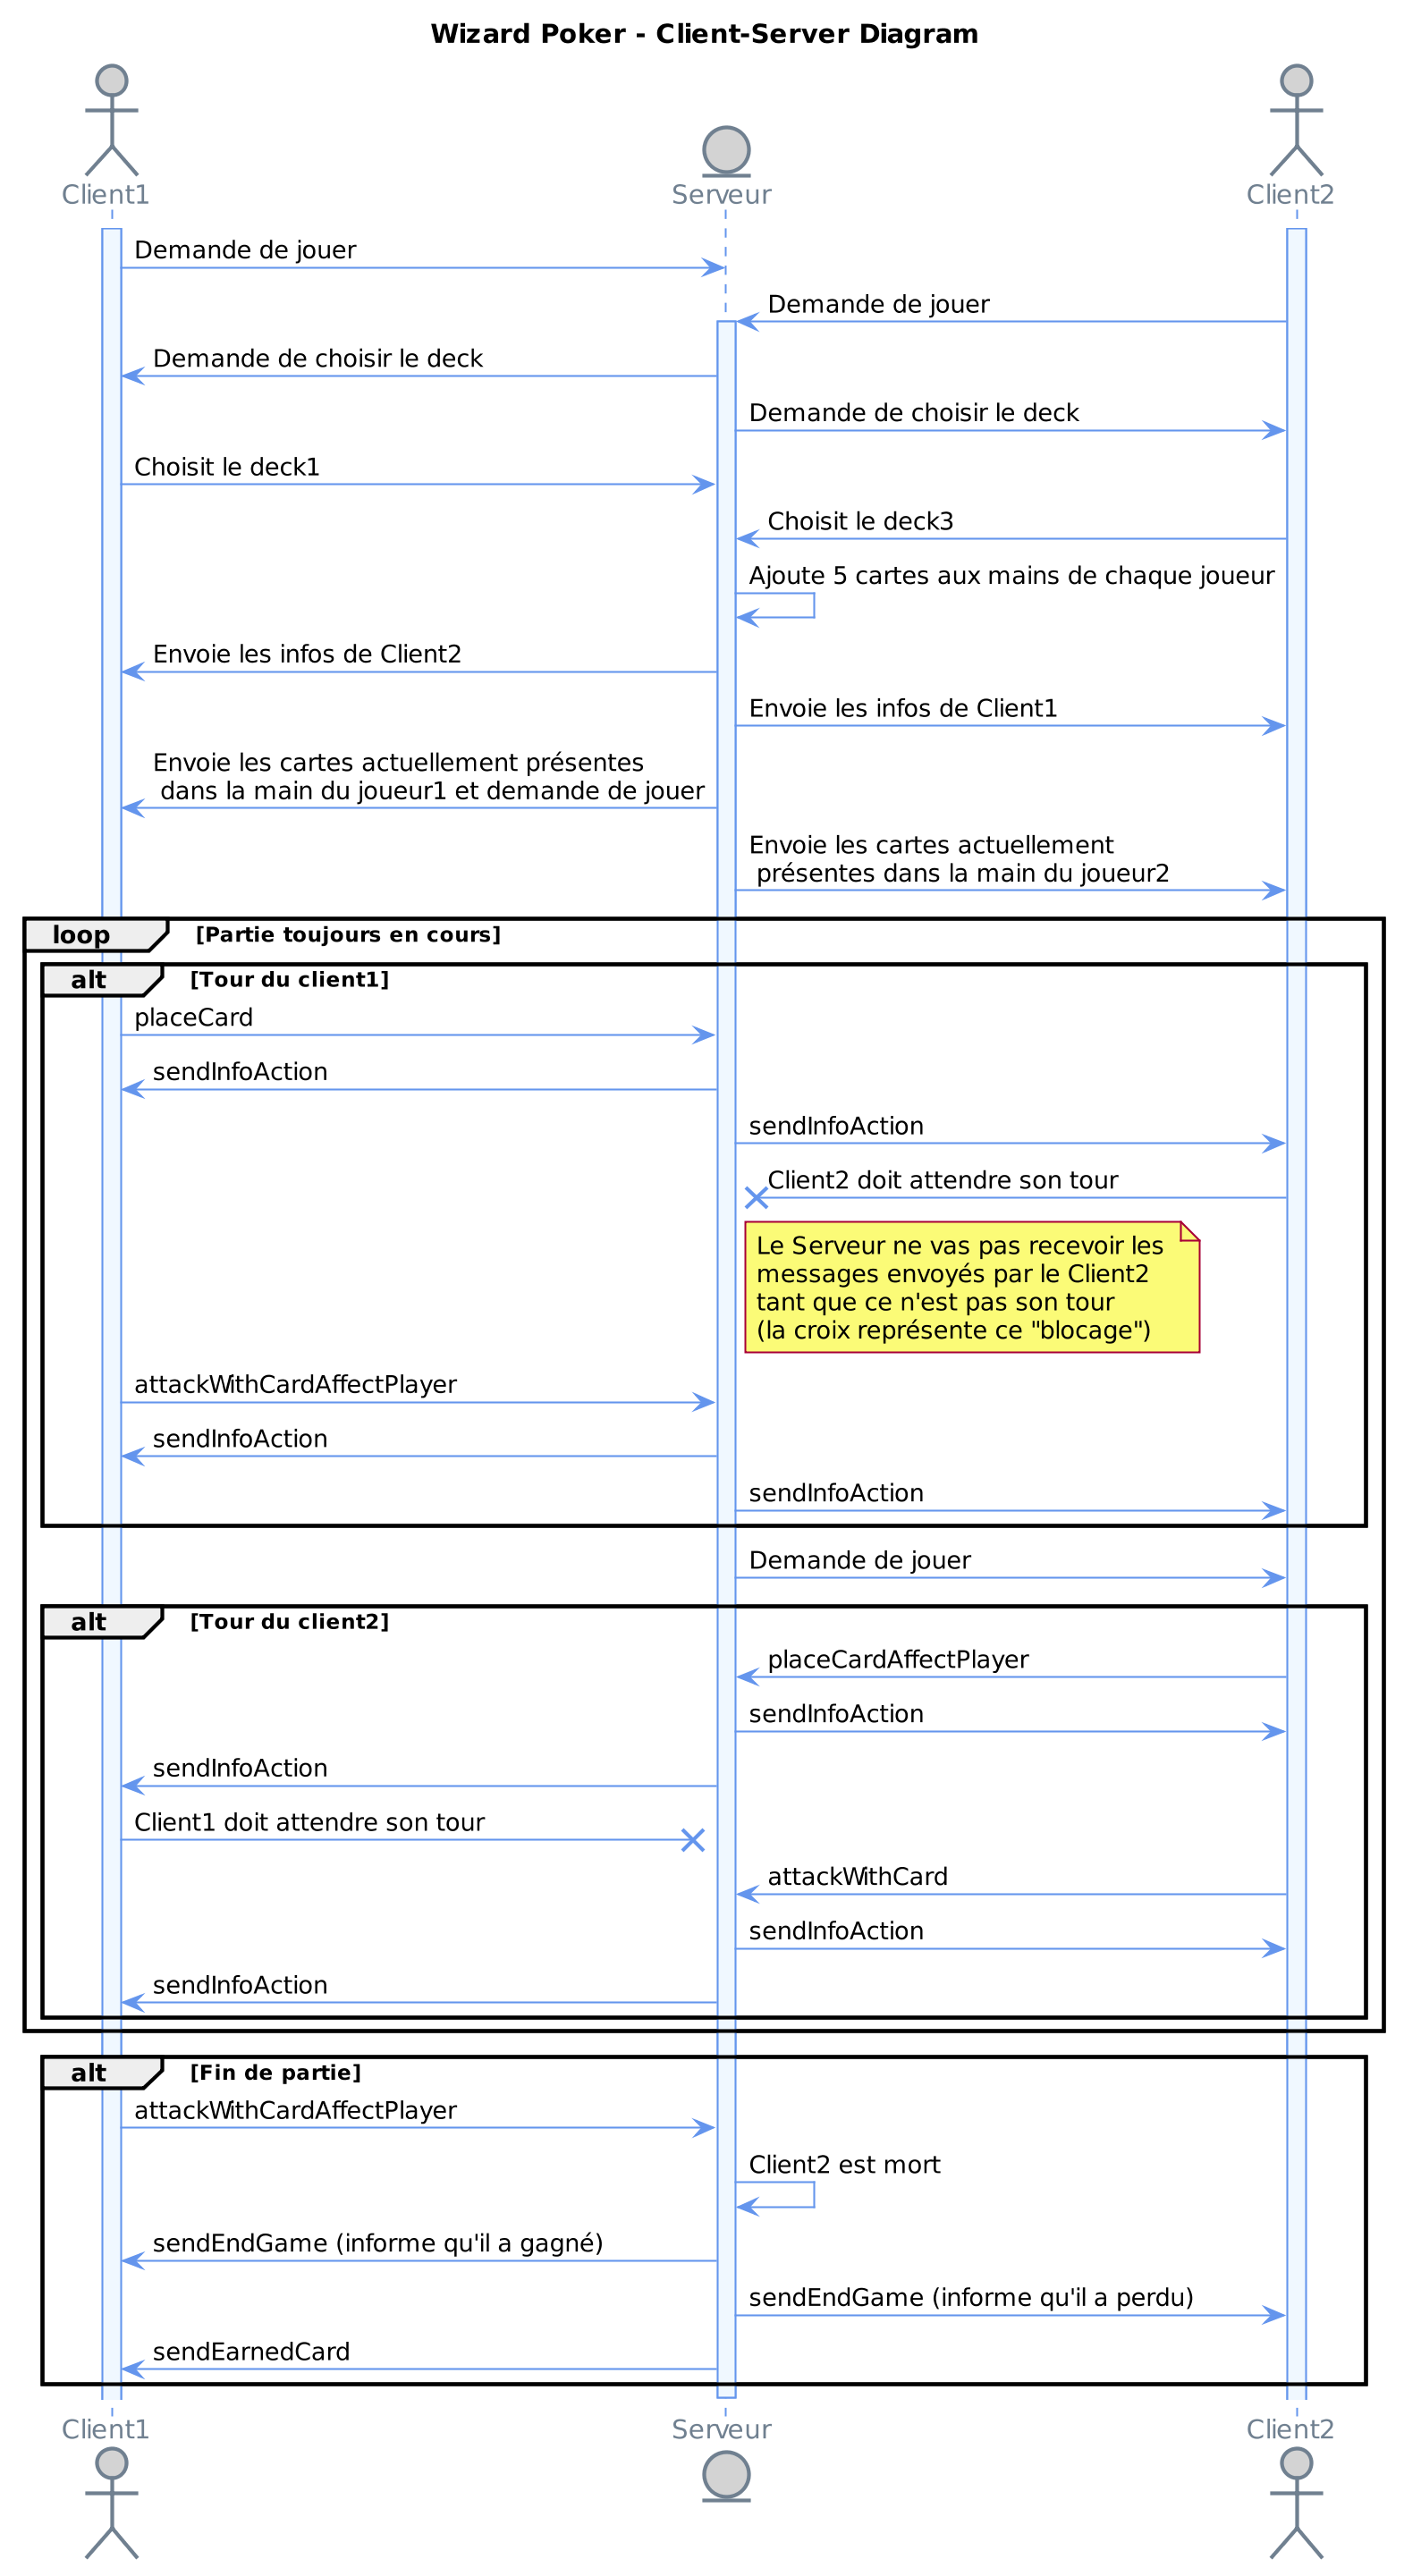
\includegraphics[width=1\textwidth]{assets/uml/UseCaseDiagram.png}
  \caption{\label{fig:usecasebesoin} Use Case Diagram}
\end{figure}

\subsubsection*{Créer un compte lié à un pseudo}

\index{Compte}
\index{Pseudo}
Tout visiteur aura la possibilité de se créer un compte
lié à un \gls{pseudo} (si ce dernier est disponible) afin de pouvoir
accéder pleinement au jeu.


\subsubsection*{Se connecter à son compte}
Le joueur devra se connecter à son compte s'il souhaite effectuer
les différentes actions répertoriées ci-dessous.\\
\underline{Pré-conditions:} 
 Avoir un compte.\\
\underline{Post-conditions:} 
 Être connecté.\\
\underline{Cas général:} 
 Le programme vérifie que le pseudo et le mot de passe sont corrects pour permettre à l'utilisateur de profiter des fonctionnalités de l'application.\\
\underline{Cas exceptionnels:} 
 Nom d'utilisateur et/ou mot de passe erroné(s).\\

\subsubsection*{Consulter sa collection de cartes}

\index{Collection}
Le joueur peut consulter l'ensemble des cartes présentes dans sa
\gls{collection}. Pour rappel, il devra au préalable s'être connecté.\\
\underline{Pré-conditions:} 
 Être connecté.\\
\underline{Post-conditions:} 
 Les cartes sont affichées.\\
\underline{Cas général:} 
 Lorsque le joueur désire consulter ses cartes, l'application doit charger les cartes gagnées grâce à ses victoires mais également les 100 cartes reçues à l'inscription.\\
\underline{Cas exceptionnels:} 
 Aucun.\\

\subsubsection*{Gestion de decks}

\index{Deck}
Plusieurs actions peuvent être effectuées sur les decks telles
qu'en supprimer un ou plusieurs, les consulter, les modifier ou tout
simplement en créer un nouveau.\\
\underline{Pré-conditions:} 
 Avoir au moins un deck.\\
\underline{Post-conditions:} 
 Affichage, modification, suppression ou création d'un deck.\\
\underline{Cas général:} 
 Le joueur demande à voir la liste de ses decks pour organiser ses cartes et créer une stratégie pour la partie.  Il peut créer, supprimer et modifier les decks.  L'application doit vérifier que le joueur a toujours au moins un deck.\\
\underline{Cas exceptionnels:} 
 Un cas exceptionnel pourrait arriver lorsque le joueur n'a pas de deck.  Mais nous ferons tout pour que ça n'arrive pas.  Il n'y a donc pas de cas exceptionnels.\\

\subsubsection*{Gérer une liste d'amis}

\index{Liste d'amis}
Chaque joueur aura une liste d'amis avec lesquels il pourra
interagir s'il le souhaite. Il pourra donc ajouter ou supprimer un ami de sa liste.\\
\underline{Pré-conditions:} 
 Être connecté.\\
\underline{Post-conditions:} 
 Voir et modifier sa liste d'amis.\\
\underline{Cas général:} 
 Affichage de la liste ou modification de celle-ci.\\
\underline{Cas exceptionnels:} 
 Aucun.\\

\subsubsection*{Discuter avec ses amis}

\index{Tchat}
Le joueur pourra, à tout moment, parler avec un de ses amis
actuellement connectés. Pour cela, un \gls{tchat} sera mis à la disposition
du joueur.  Le joueur pourra donc à tout moment communiquer avec ses amis par
messagerie instantanée. Cependant un joueur ne pourra communiquer qu'avec
une personne à la fois.\\
\underline{Pré-conditions:} 
 Être connecté et avoir au moins un ami dans sa liste qui est connecté.\\
\underline{Post-conditions:} 
 Une conversation s'établit entre les deux personnes.\\
\underline{Cas général:} 
 Une bulle de conversation s'ouvre.\\
\underline{Cas exceptionnels:} 
 Une perte de connexion fermera la conversation entre deux personne.\\

\subsubsection*{Proposer une partie à un ami}

Si le joueur le souhaite, il peut proposer une partie à un de ses
amis connectés. Ce dernier est libre d'accepter ou non cette demande.
S'il l'accepte la partie est lancée entre les deux joueurs.\\
\underline{Pré-conditions:} 
 Être connecté et disponible et avoir un ami connecté disponible (pas en partie).\\
\underline{Post-conditions:} 
 Invitation à jouer envoyée à l'ami choisi.\\
\underline{Cas général:} 
 Lancement d'une partie contre cet ami.\\
\underline{Cas exceptionnels:} 
 Aucun.\\
 

\subsubsection*{Trouver un adversaire pour un duel}

Lorsqu'un joueur voudra lancer une partie, le jeu trouvera
automatiquement un adversaire dans la liste des personnes
connectées. Le choix de l'adversaire est totalement aléatoire.\\
\underline{Pré-conditions:} 
 Être connecté et avoir au moins un deck formé (cela devrait être tout le temps le cas, comme expliqué dans la partie relative aux Deck).\\
\underline{Post-conditions:} 
 Changement de statut : de "disponible" à "en partie".\\
\underline{Cas général:} 
 La partie se lance contre l'adversaire trouvé.\\
\underline{Cas exceptionnels:} 
 Aucun adversaire n'a été trouvé.\\

\subsubsection*{Consulter le classement}

\index{Classement}
Le classement va permettre de classer les joueurs en fonction de
leur nombre de victoires et de défaites. Ce classement se
basera donc sur un ratio victoires/défaites.\\
\underline{Pré-conditions:} 
 Être connecté.\\
\underline{Post-conditions:} 
 Affichage du classement.\\
\underline{Cas général:} 
 La liste des cartes des joueurs est chargée depuis la base de donnée et est affichée au joueur.\\
\underline{Cas exceptionnels:} 
 Aucun.\\

\subsection{Exigences non fonctionnelles}
\label{sec:exi-nonfonc}

Les exigences non fonctionnelles, n'étant, pour la plupart, pas indispensables au fonctionnement de l'application, elles ne seront pas mises en œuvre en priorité.


\subsubsection*{Ergonomie}
Il s'agit de créer un jeu qui sera simple d'utilisation et facilement compréhensible pour un utilisateur n'ayant jamais joué à un jeu de ce genre.
\medbreak
Une des solutions trouvées est de rendre l'interface intuitive à l'aide de ``boutons'' décrivant exactement leur utilité ou encore à l'aide d'un rapide tutoriel expliquant au joueur, après la création de son compte, les différentes caractéristiques du jeu.


\subsubsection*{Design}
Le design est l'apparence qu'aura l'interface graphique. Elle est en partie liée au point précédent puisqu'une interface attrayante permettra à l'utilisateur de facilement repérer les différentes possibilités offertes par le jeu en plus d'en apprécier l'esthétique.
\medbreak
Le design est un large ``domaine'' : c'est-à-dire qu'il définit aussi bien l'apparence du jeu  que les effets spéciaux (comme les différents sons et/ou musiques pouvant être intégrés au jeu).


\subsubsection*{Amusement}
Un des objectifs, même s'il est loin d'être le plus prioritaire dans ce contexte, est de créer une application attirante. Par ailleurs, plus les utilisateurs s'amuseront en jouant au Wizard Poker, plus elle sera attractive.


\subsection{Exigences de domaine}
\label{sec:exi-dom}

Le domaine du jeu vidéo laissant beaucoup de liberté, chaque créateur a la possibilité de développer son univers, ses concepts, etc.  Cependant, les jeux doivent permettre à leurs utilisateurs de trouver du plaisir ou une certaine forme de satisfaction.  Il faut donc éviter, par exemple, qu'un joueur soit interrompu durant sa partie.  Les exigences du domaine ne sont pas nombreuses mais il peut être compliqué de toutes les satisfaire.

\medbreak

Nous mettons en place ici un jeu de cartes et ce type de jeu impose quelques contraintes.  En effet, il faut que le jeu soit le plus équilibré possible : il faut donc, par exemple, éviter que certaines cartes ne soient trop "fortes" par rapport à d'autres.  En ce qui concerne le temps de jeu d'une partie, il faut veiller à ce que ce ne soit ni trop long (et donc éviter les abandons de partie), ni trop court (pour ne pas rendre le jeu lassant). Finalement, pour ce qui est de la durée de vie globale du jeu, il faut faire en sorte qu'il y ait un nombre conséquent de cartes afin que les joueurs puissent régulièrement renouveler leur collection.

\medbreak

En conclusion, on peut dire qu'un utilisateur attend un jeu équilibré et une stabilité acceptable (voire infaillible côté serveur).  Nous nous concentrerons dans un premier temps sur ce deuxième point.



\section{Besoins du système}
\label{sec:besoins-sys}

\subsection{Exigences fonctionnelles}
\label{sec:exi-fonc-sys}

Dans cette partie, nous nous intéresserons à ce que l'application doit
faire pour interagir avec l'utilisateur et lui proposer toutes les
actions mentionnées ci-dessus (voir \ref{sec:exi-fonc}). Nous détaillerons
donc comment le système réalisera toutes ces tâches.

\subsubsection*{Connexion}

Connection avec IPv4... avec socket etc

un thread est initialisé...

\subsubsection*{Login et enregistrement}

Les utilisateurs peuvent se connecter ou s'enregistrer à travers la
fenêtre de login, réalisée avec \texttt{ncurses} et introduire leur
pseudonyme et mot de passe. Ces informations sont transmises au serveur
qui vérifie si celles-ci sont correctes.


\subsubsection*{Classement}

Tout joueur inscrit peut consulter le classement. Celui-ci est donné en
vérifiant toutes les victoires et défaites de chaque joueur. La liste
est affichée par ordre décroissant sur le ratio victoires/défaites.

\subsubsection*{Sauvegarde. Sérialisation/Désérialisation}

Les données des joueurs propres au jeu (decks,
collections de cartes, nombres de victoires et défaites etc) sont
enregistrées à chaque déconnexion des joueurs. La prochaine fois que
l'utilisateur se connecte, il aura toutes ses données comme avant.

Cela est possible grace a la sérialisation de l'information au format
JSON\footnote{JavaScript Object Notation}. Ce n'est pas une vraie base
de données mais bien un fichier texte qui est sauvegardé dans le
serveur. Toutes les complexités liées aux bases de données sont donc éliminées pour
ce simple jeu.





\subsection{Exigences non fonctionnelles}
\label{sec:exi-nonfonc-sys}

Les exigences non fonctionnelles décrivent le comportement de
l'application.

\medbreak

Le système doit tout d'abord être robuste et stable, c'est-à-dire
gérer toutes les erreurs possibles, éviter les crashs et les éventuelles
déconnexions.

\medbreak

Par ailleurs, il doit être agréable d'utilisation pour le joueur
(ergonomique et esthétique) et garantir que celui-ci ne puisse
pas tricher pendant une partie.

\medbreak

En résumé, le système doit être robuste, stable, sûr, et excessivement amusant. Des
heures de détente, en toute sécurité, sont assurées à tout utilisateur du jeu.

\subsection{Design et fonctionnement du système}
\label{sec:design}

Afin de mieux présenter le fonctionnement du programme, voici quelques
diagrammes sur lesquels nous nous baserons lors du
développement du Wizard Poker.

\medbreak

Le diagramme de classe présenté à la Figure \ref{fig:class} sera celui sur lequel nous nous baserons le plus lors de l'écriture du code.

\begin{sidewaysfigure}[ht]
  \centering
  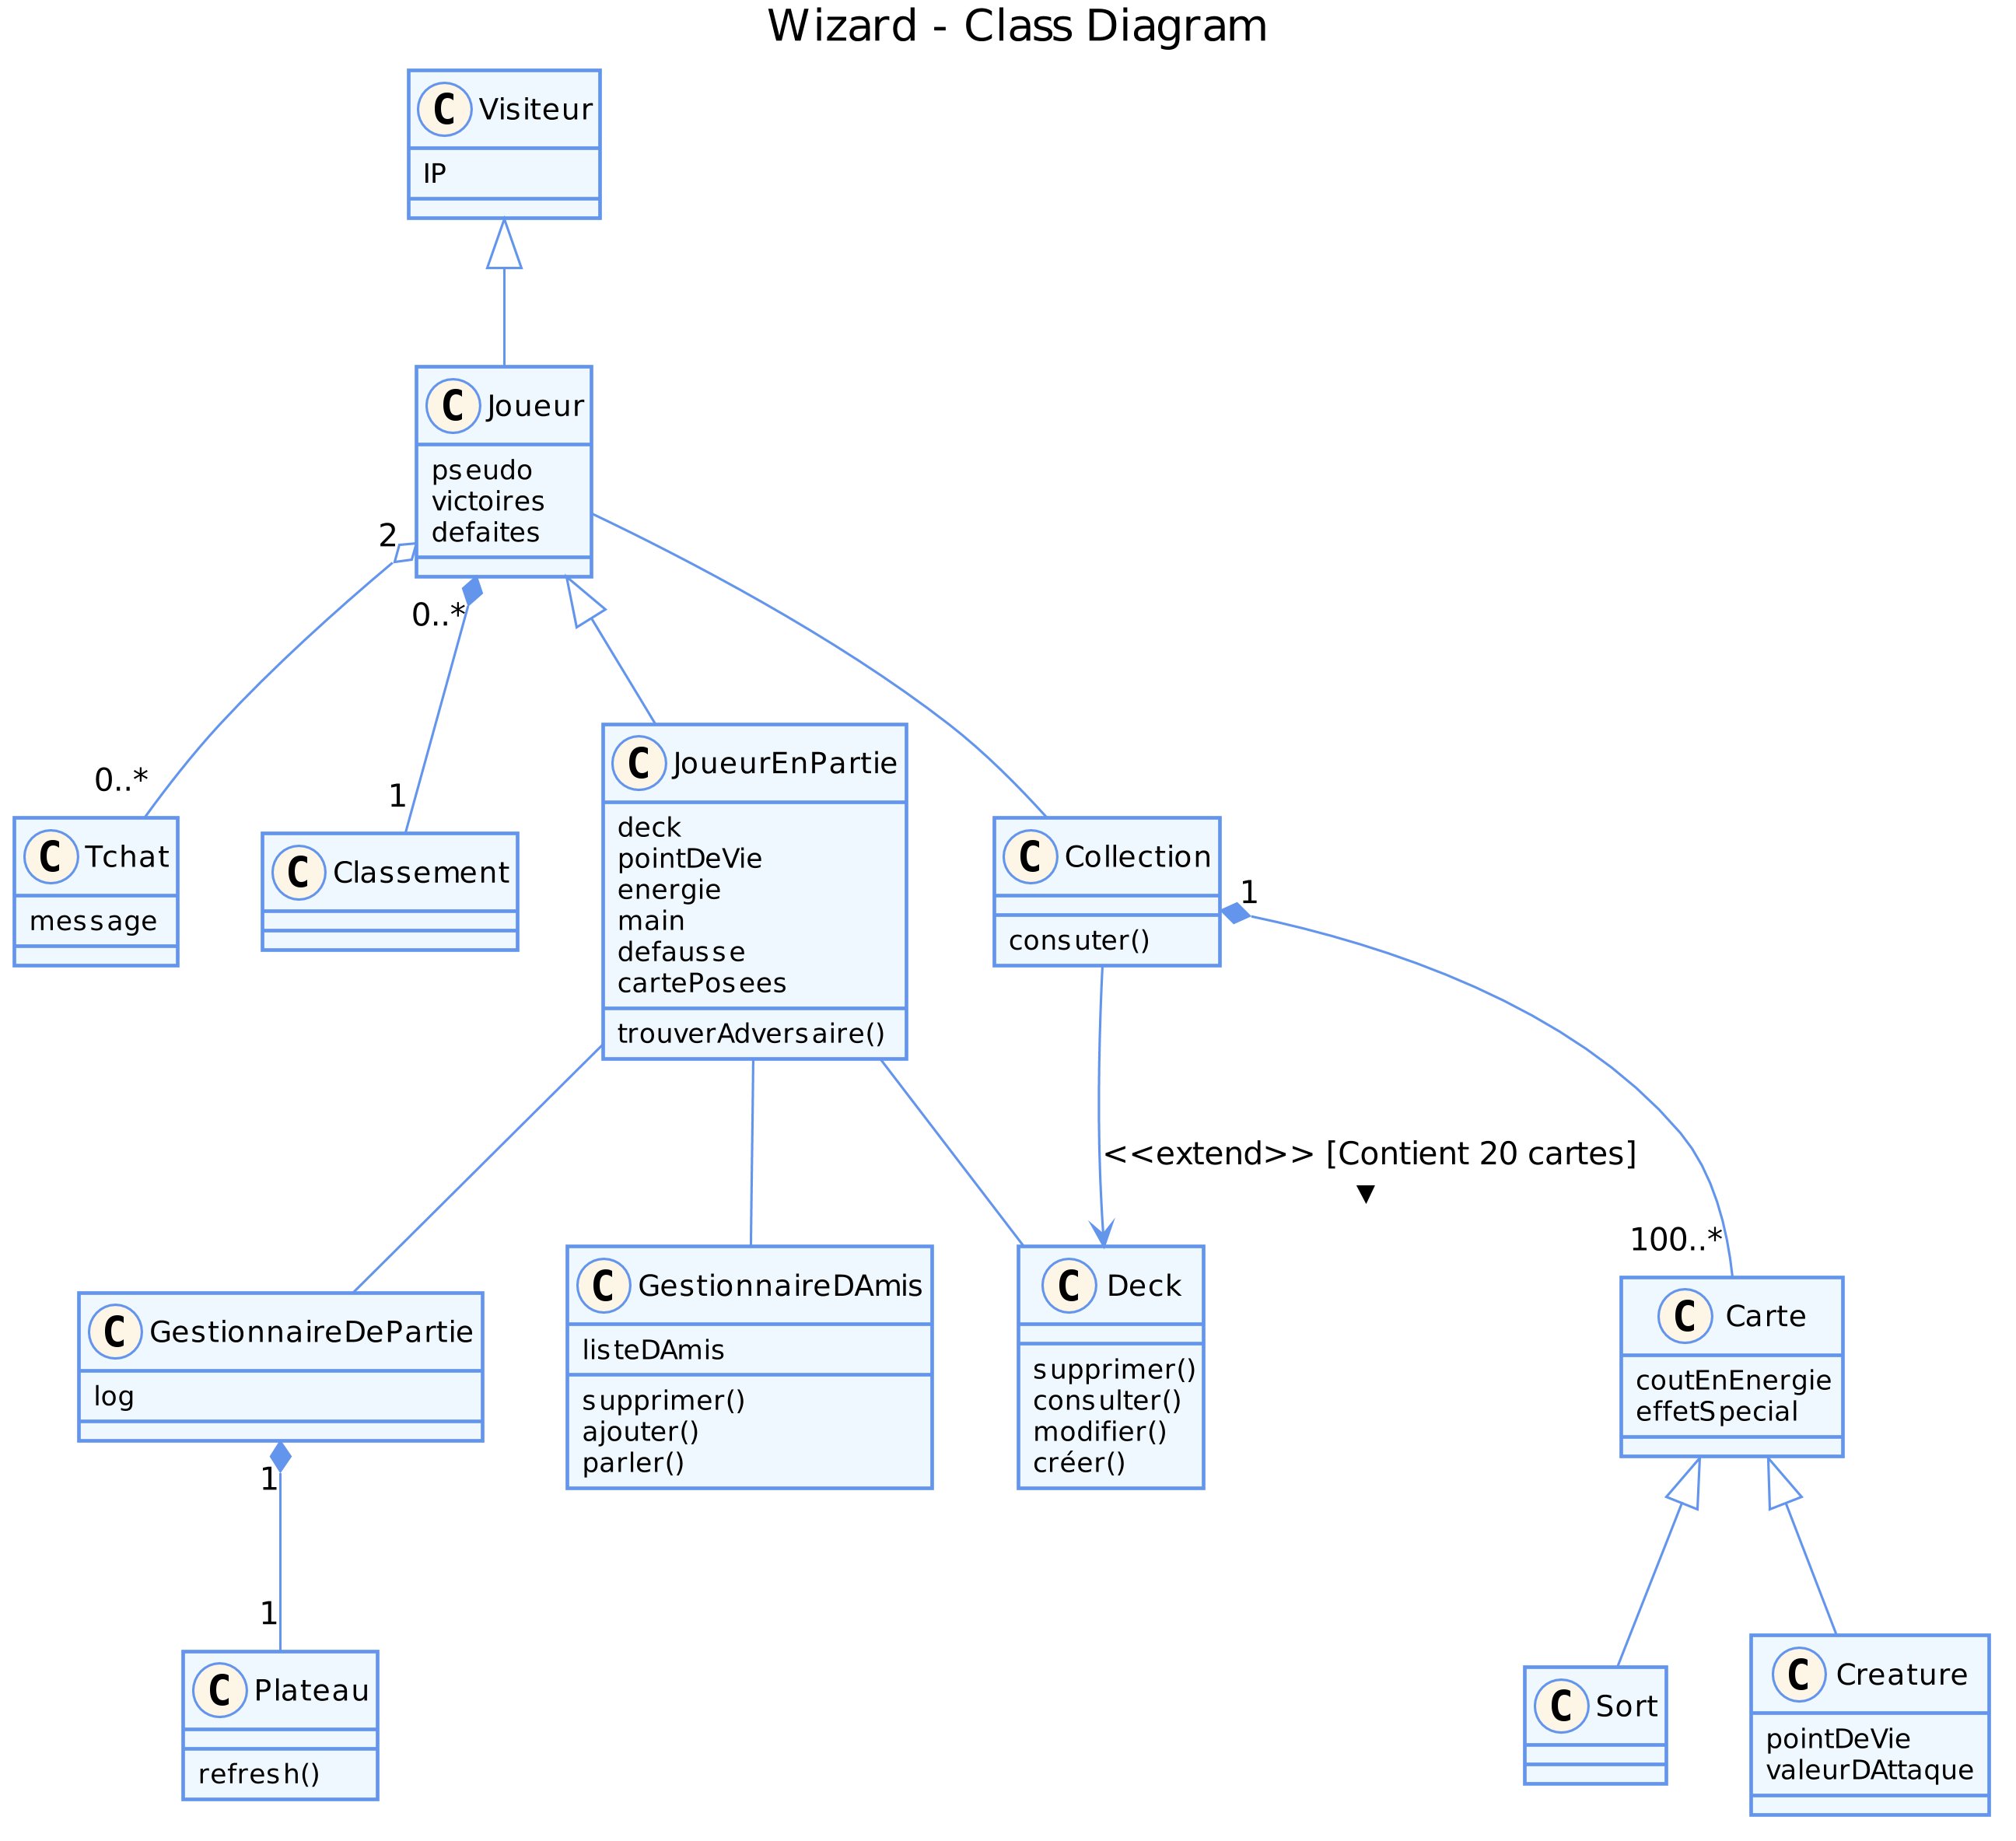
\includegraphics[width=0.8\textwidth]{assets/uml/ClassDiagram1.png}
  \caption{\label{fig:class} Diagramme de classes}
\end{sidewaysfigure}

\begin{sidewaysfigure}[ht]
  \centering
  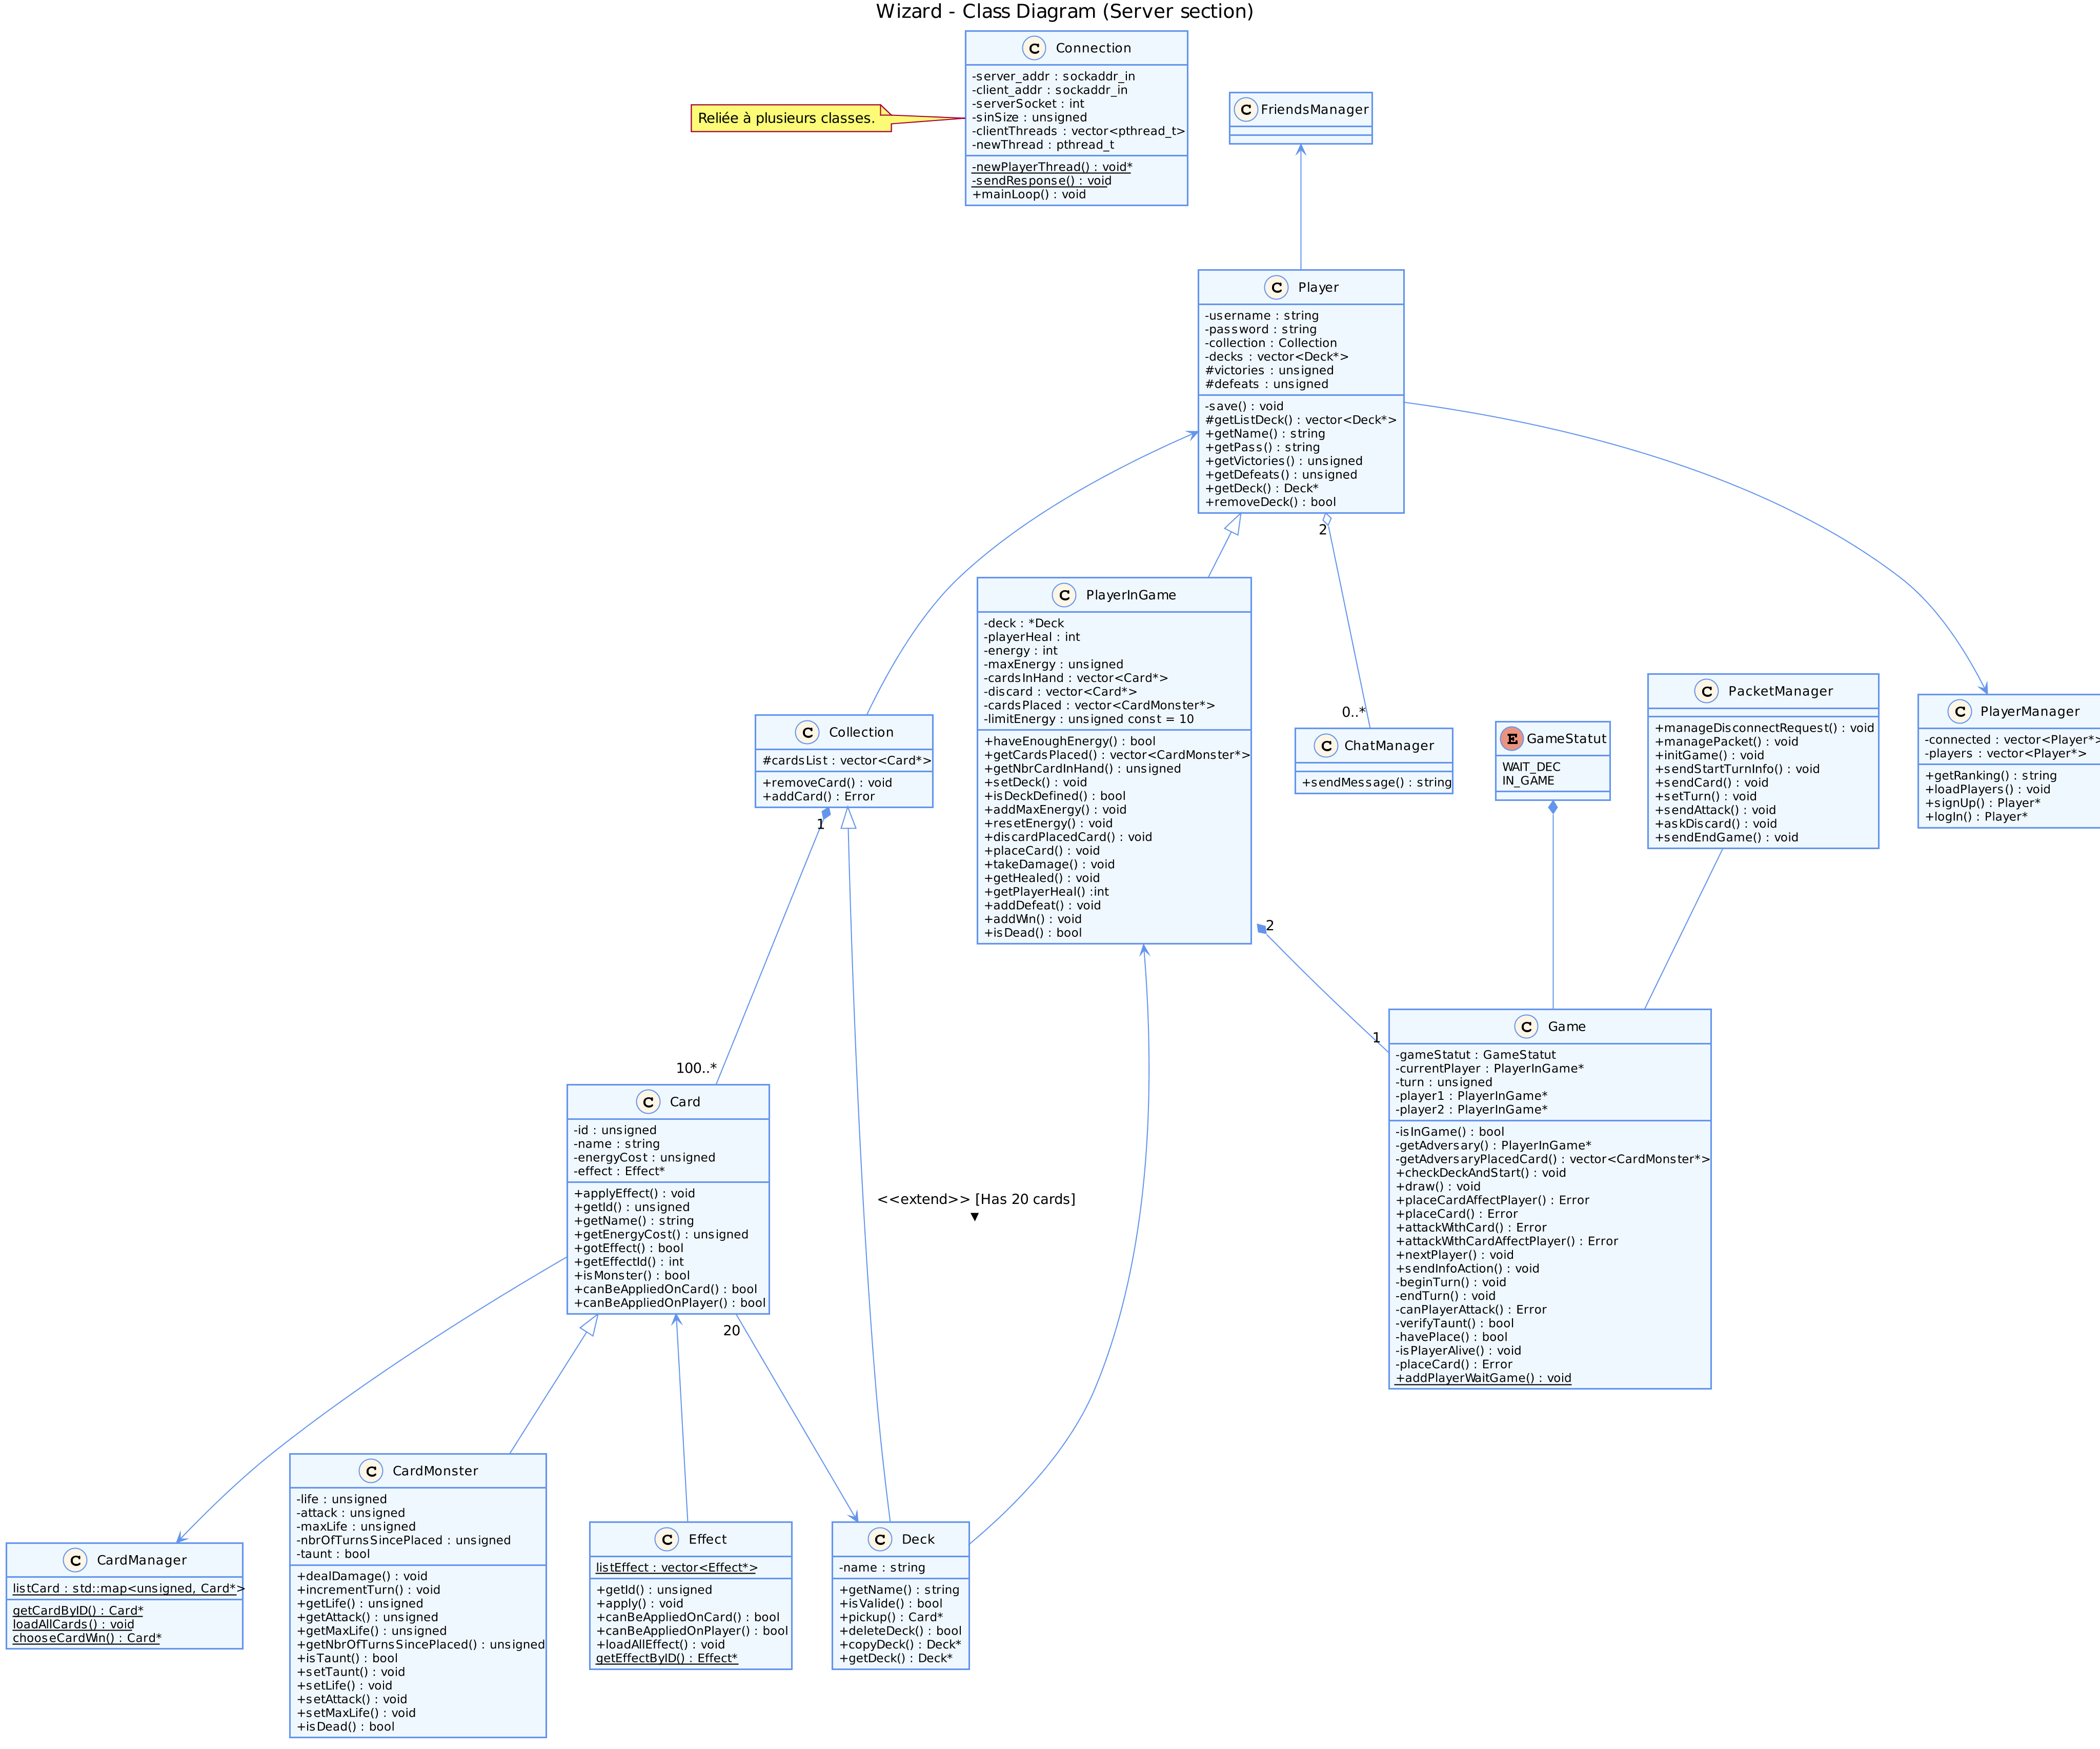
\includegraphics[width=0.95\textwidth]{assets/uml/ClassDiagram2.png}
  \caption{\label{fig:class} Diagramme de classes}
\end{sidewaysfigure}

\subsubsection{Diagramme client/serveur}

\index{Initialiser une partie}
Le diagramme client/serveur, présenté à la Figure \ref{fig:seq}, vise à montrer la manière dont un joueur va
pouvoir jouer une partie.

\begin{figure}[ht]
  \centering
  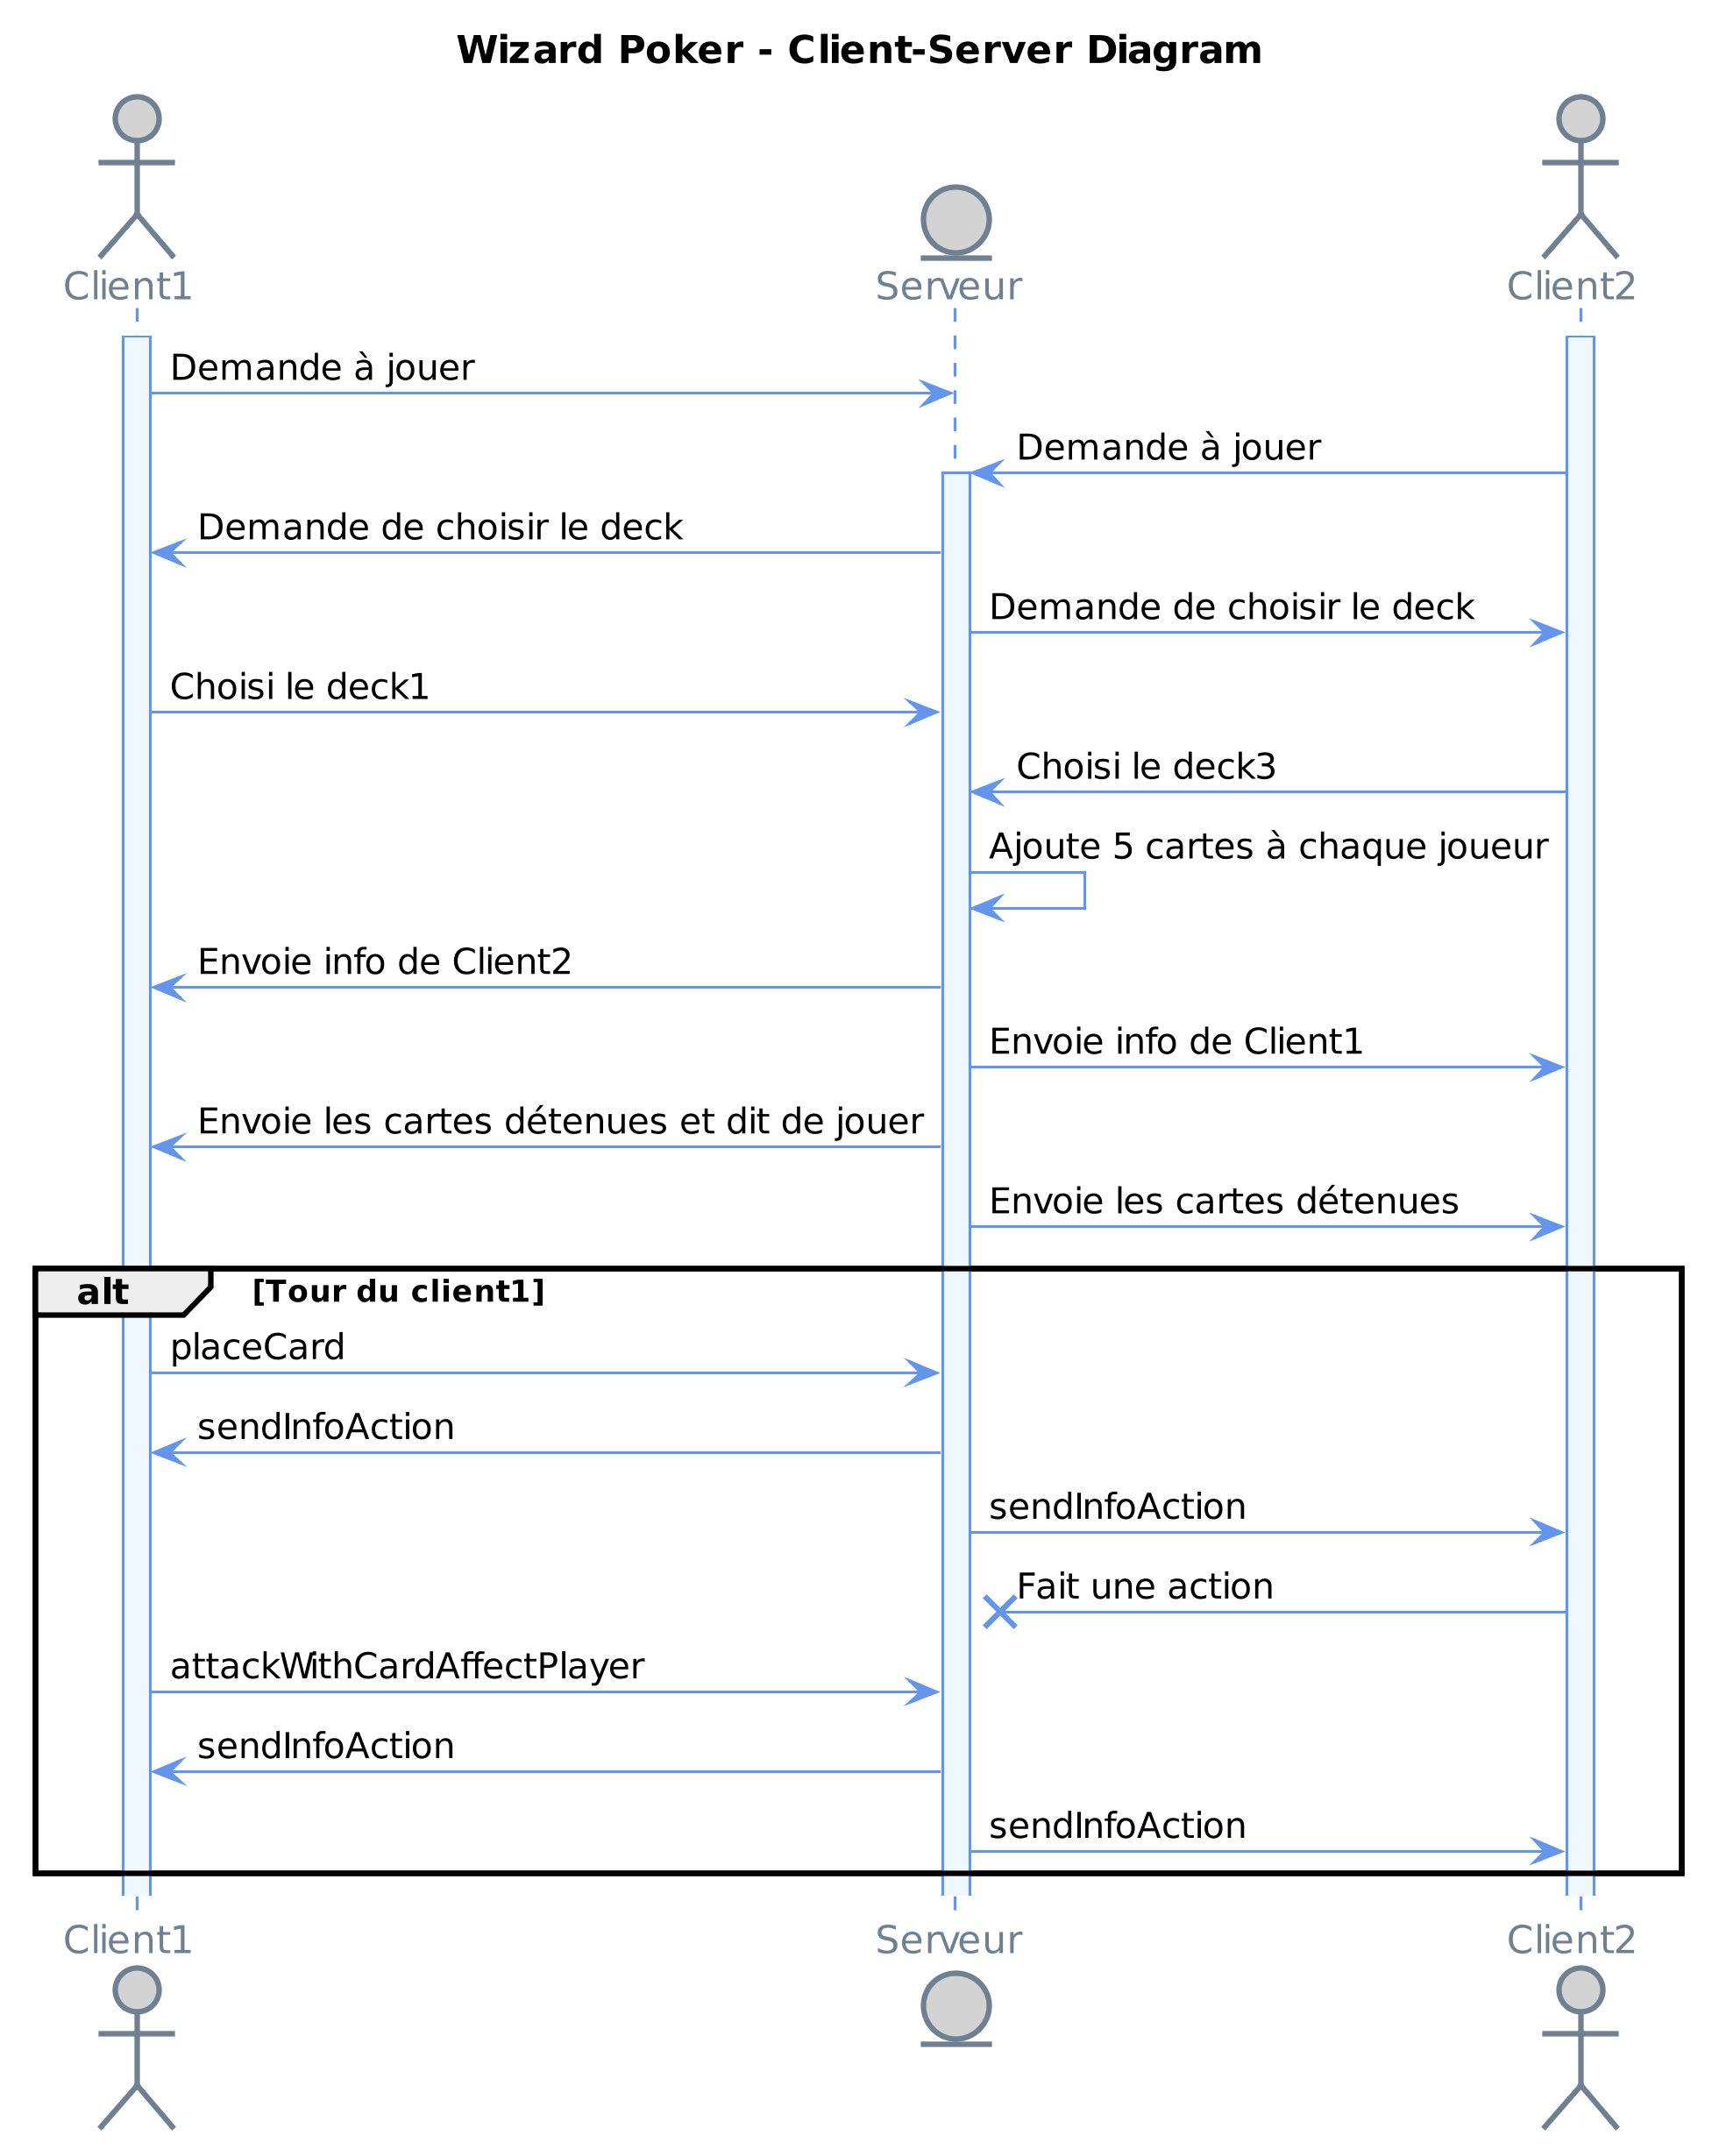
\includegraphics[width=1\textwidth]{assets/uml/ClientServerDiagram.png}
  \caption{\label{fig:seq} Diagramme client/serveur}
\end{figure}

\subsubsection{Diagrammes d'activité}
L'objectif de ces trois diagrammes d'activité, présentés aux Figure \ref{fig:act1}, \ref{fig:act2}, \ref{fig:act3}, est de décrire le déroulement de la partie.
\begin{figure}[ht]
  \centering
  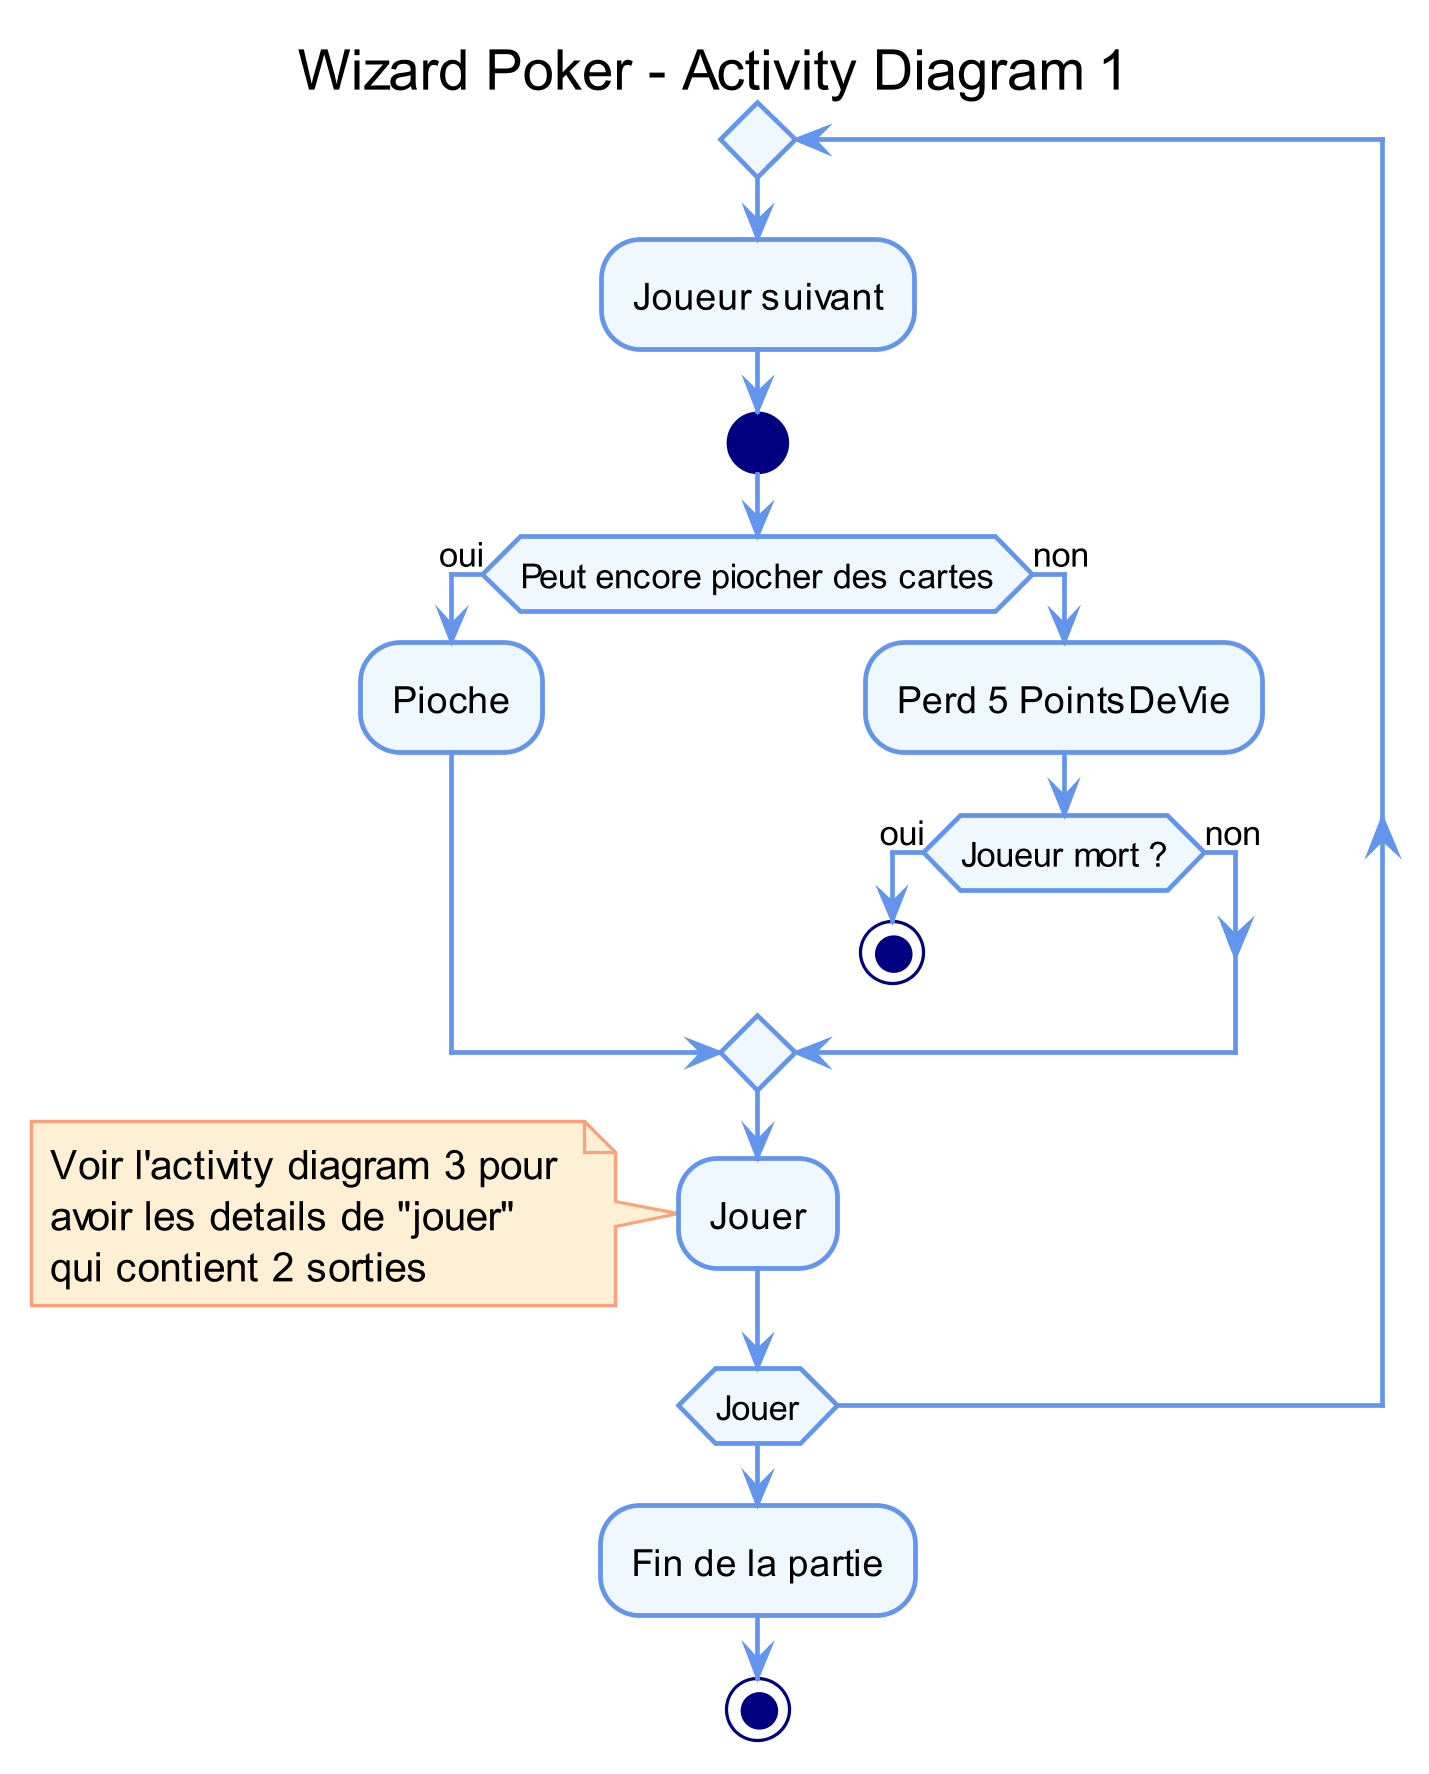
\includegraphics[width=0.7\textwidth]{assets/uml/ActivityDiagram1.png}
  \caption{\label{fig:act1} Diagramme d'activité 1}
\end{figure}

\begin{figure}[ht]
  \centering
  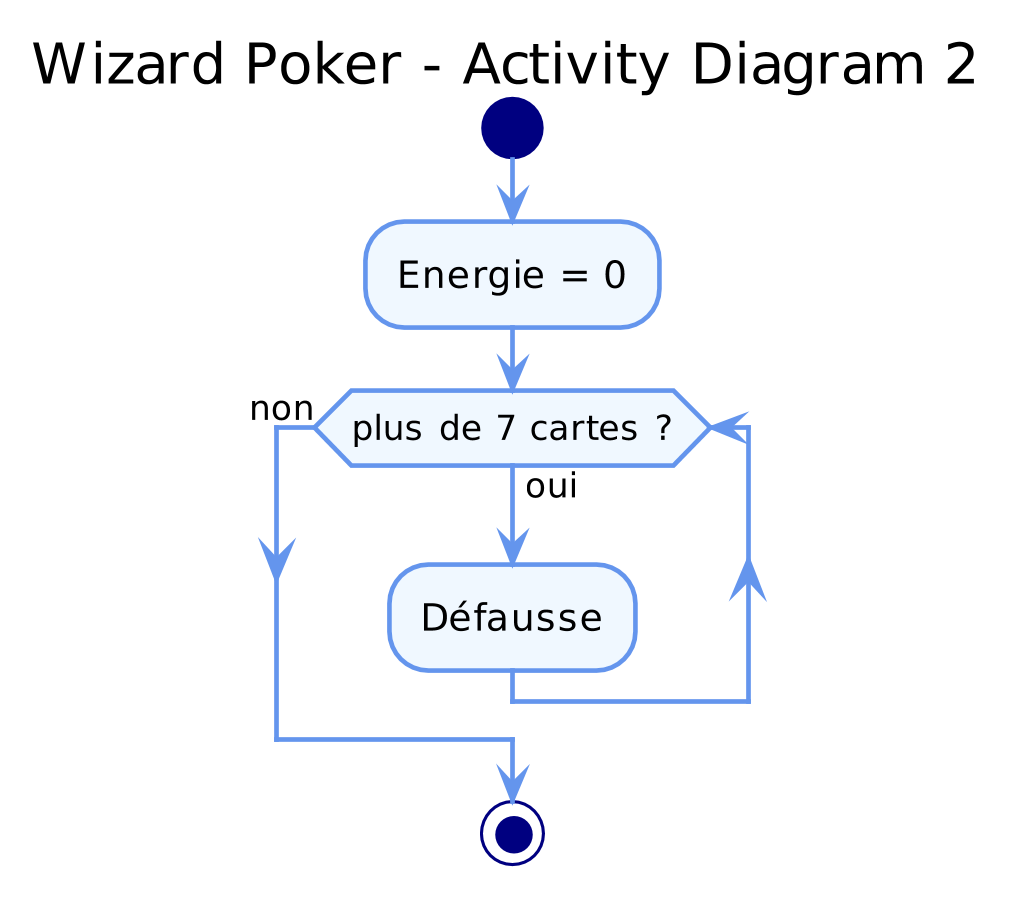
\includegraphics[width=0.5\textwidth]{assets/uml/ActivityDiagram2.png}
  \caption{\label{fig:act2} Diagramme d'activité 2}
\end{figure}

\begin{sidewaysfigure}[ht]
  \centering
  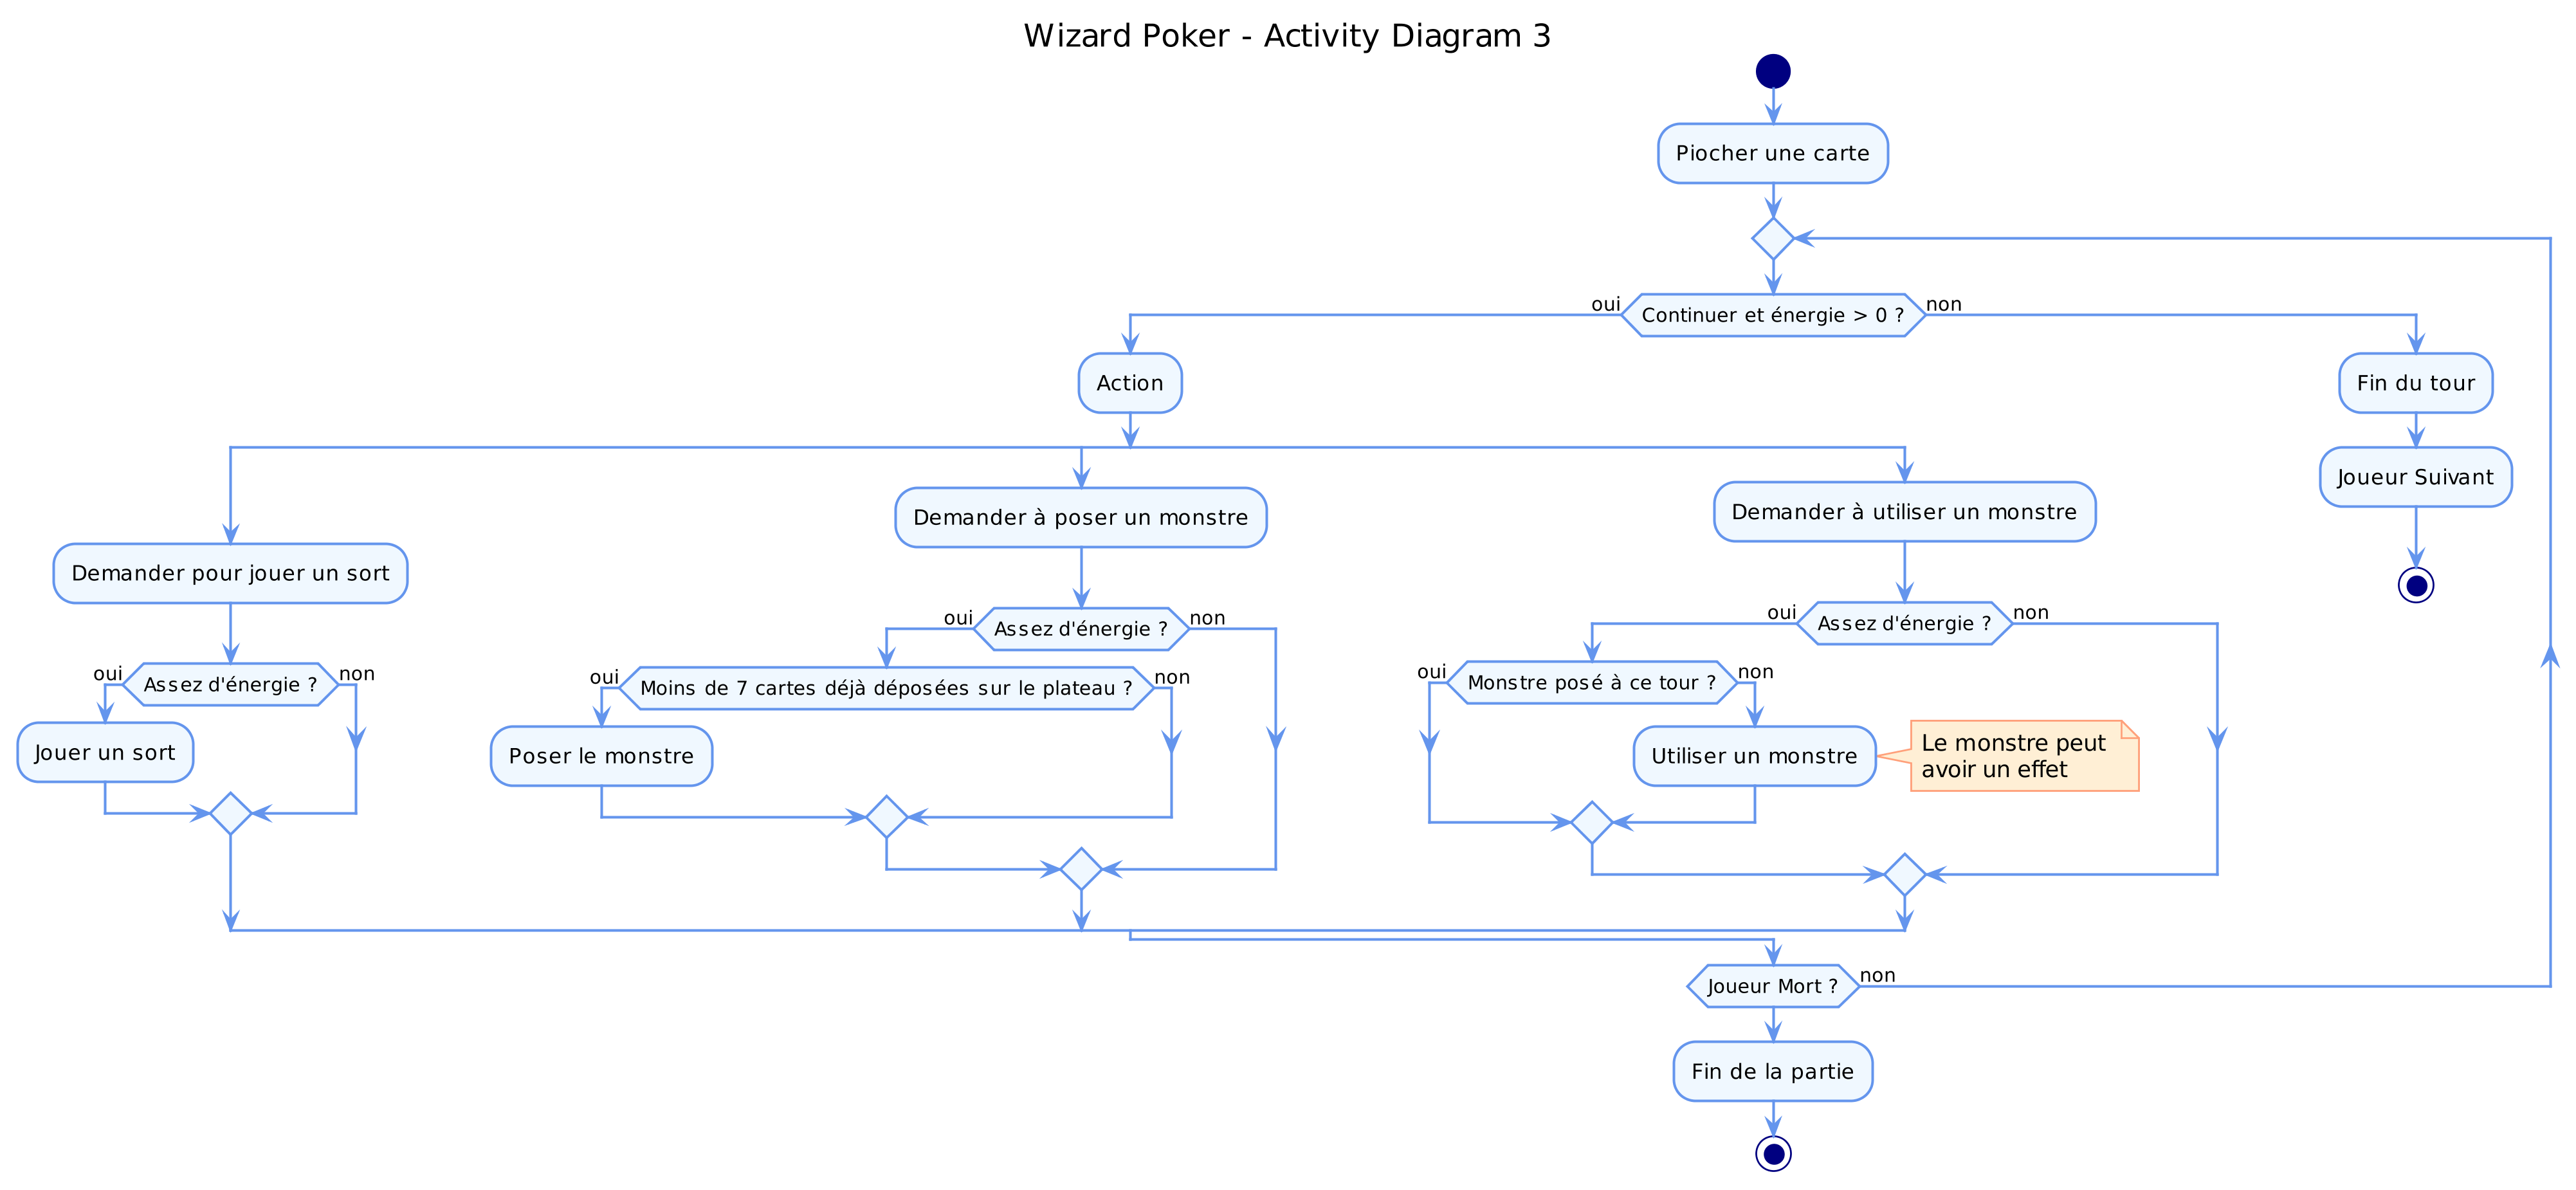
\includegraphics[width=1\textwidth]{assets/uml/ActivityDiagram3.png}
  \caption{\label{fig:act3} Diagramme d'activité 3}
\end{sidewaysfigure}

\clearpage
\printindex

\end{document}
